\chapter{Návrh testovací laboratoře}
Pro testování všech výrobků společnosti Conel nejdříve navrhnu strukturu testovací laboratoře. Testovací laboratoř bude LAN síť obsahující všechny testované výrobky společnosti Conel, různá příslušenství připojené k jednotlivým výrobkům, testovací server a dva konfigurovatelné switche. Fyzicky bude pro testovací síť vyroben rack s půdorysem asi 60cm na 80cm a výškou jeden a půl metru. Konfigurovatelné switche budou umístěny ve spodní části racku. Na dvouch protilehlých částech budou v patrech namontovány DIN lišty na které se budou přidělávat testované routery, či různá další zařízení potřebná k samotnému testování.

\section{Testovací server}
Jádrem testovací laboratoře bude server na kterém poběží všechny aplikace pro samotné testování a reprtování výsledků. Testovací server je připojen ke všem zařízením v testovací sítí a odděluje tyto zařízení od firemní sítě. Fyzicky může testovací server být umístěn jinde nežli uvnitř racku, jelikož ho s testovací sítí propojují pouze dva ethernetové kabely.

\begin{figure}[h]
  \centering
  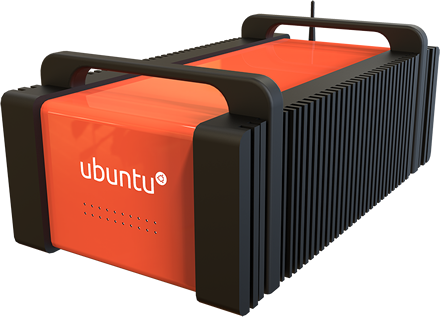
\includegraphics[width=.3\LW]{ubuntu}
  \caption{Ubuntu server}
  \label{fig:ubuntu}
\end{figure}

\subsection{Hardwerová výbava testovacího serveru}
Testovaci server bude počítač s parametry procesor Intel core i7, 16GB RAM a 256GB SSD diskem. V případě potřeby budou pro starší logy a přeložené firmwary doplněny další klasické magnetické disky. Pro účely testování bude server osazen dvěma gigovými ethernetovými karty pro komunikaci s testovanými výrobky a jednou gigovou ethernetovou kartou pro konektivitu serveru do firemní sítě. Server dále má osazeno jedno WiFi rozhraní pro testování WiFi konektivity výrobků.

\subsection{Softwarová výbava testovacího serveru}
Operační systém tohoto serveru jsem zvolil Linuxovou distribuci Ubuntu, jelikož operační systém Ubuntu je používán jako referenční systém při vývoji. Nasazena bude verze Ubuntu Server 14.04.1 LTS s prodlouženou podporou na pět let. Na serveru bude umístěna databáze uchovávající všechny informace o testotování a webová aplikace zobrazující výsledky z testování. Databázový systém použitý k uchovávání výsledku bude MySQL. Pro fungování webové aplikace bude na server nainstalován Apache server a PHP. Spouštění testů obsluhuje testovací aplikace testlab, která je umístěna na testovacím serveru. Na server se také instaluje řada malých samostatných programů tvořící API pro zjednodušní psaní jednotlivých testů. Pogramy instalované na server, které jsou využívány programem testlab a testovacím api budou popsány u programů, kde jsou použity. Na serveru bude dále umístěna kopie vzdáleného repozitáře pro rychlejší stahování zdrojových kódu testovaných projektů při samotném testování. V dalších fázích vývoje testovacího zařízení by na tomto serveru mohl být testován systém pro monitoring routerů RSeeNet a systém pro jednoduchou správu VPN tunelů SmartCluster.

\section{Konfigurovatelné switche}
Pro připojení všech výrobků k testovacímu serveru budou použity dva konfigurovatelné 48 portové switche od firmy CISCO. Dva switche byly zvoleny z důvodu velké ceny switchů nad 48 portů. Konfigurovatelné switch budou potřeba pro možnost změny síťové infrastruktury v průběhu testů. Každý switch bude připojen k jednomu ethernetovému rozhraní serveru, dále switche budou navzájem propojeny. Nejen všechny testované výrobky, ale každé fyzické ethernetové rozhraní každého výroku bude připojeno do switche. Pomocí VLAN bude možné sítě oddělit a vytvořit požadovanou testovací síť. Do switche budou dále připojeny další pomocné zařízení použité k testování, například CISCO router.

\begin{figure}[h]
  \centering
  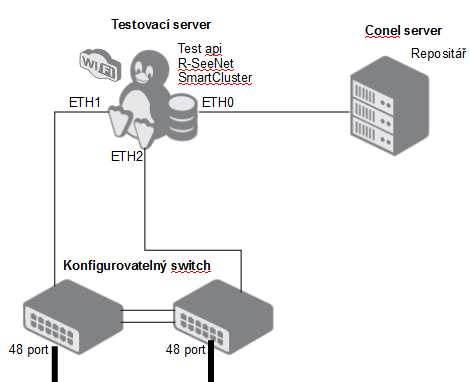
\includegraphics[width=.4\LW]{server_switch}
  \caption{Zapojení testovacího serveru a switchů}
  \label{fig:server_switch}
\end{figure}

\section{Testovaná zařízení}
Bezdrátové routery jsou zařízení které tvoří přes devadesát procent sortimentu firmy Conel a právě tato zařízení budou testovány v testovací laboratoři. Bezdrátové routery tvoří celkem čtyři modelové řady, které dále obsahují jednotlivé výrobky podle technologie bezdrátového připojení a úrovně výbavy možných rozhraní.

\subsection{Řada routerů v0}
Takzvaná nultá řada routerů obsahuje pouze dvá výrobky. Prvním výrobke je ER75i, disponující EDGE technologií, jedním ethernet rozhraním a možností osazení jednoho volitelného portu. Druhým výrobkem této řady je UR5, který se liší pouze bezdrátovou technologií. Místo EDGE technologie disponuje rychlejší UMTS technologií. Oba tyto výrobky jsou postaveny na uClinuxu a i přes jejich stáří se firmware stále udržuje. U těchto modelů bude připojeno pouze ethernet rozhraní, které bude připojeno do konfigurovatelného switche. Testování volitelného portu bude popsáno v samostanté kapitole věnující se testování volitelných portů. Jiné interface tato základní řada neobsahuje.

\subsection{Řada routerů v1}
Řada routeru v1 není od nulté řady marketingově ani koncepčně nijak oddělena. Řada je z hlediska vývoje je oddělena jelikož je založena na plnohodnotném Linuxu, namísto uCLinuxu použitém u předchoích výrobků. Řada obsahuje výrobky UR5i disponující HSPA+ technologií a drátovým routerm XR5i, který nedisponuje žádnou bezdrátovou technologií.

\begin{figure}[h]
  \begin{subfigure}[h]{0.5\LW}
    \centering
    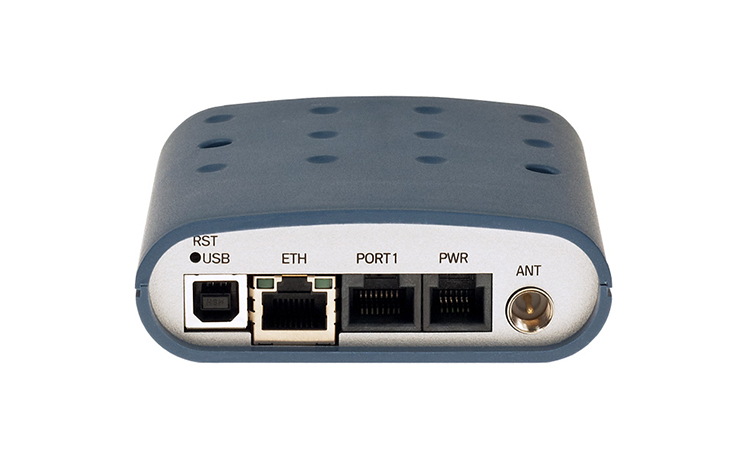
\includegraphics[width=.5\LW]{ER75i}
    \caption{ER75i v plastové krabici.}
    \label{fig:ER75i}
  \end{subfigure}
  \begin{subfigure}[h]{0.5\LW}
    \centering
    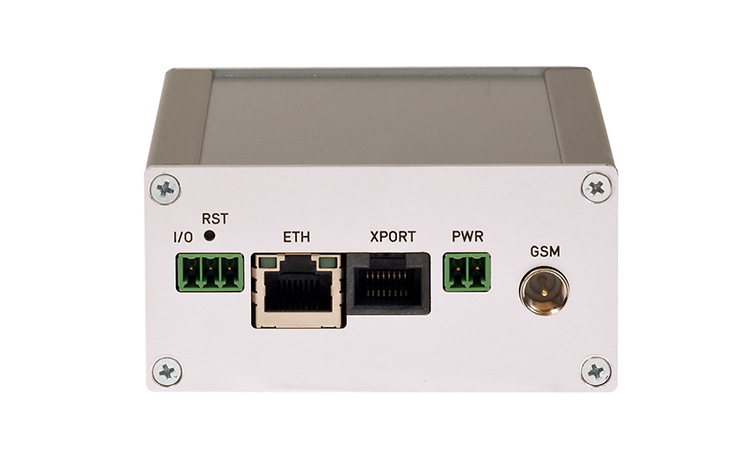
\includegraphics[width=.5\LW]{ER75i_SL}
    \caption{ER75i v kovové krabici.}
    \label{fig:ER75i SL}
  \end{subfigure}
  \caption{Příklad vzhledu řady routerů v0 a v1.}
  \label{fig:ER75i}
\end{figure}

\subsection{Řada routerů v2}
Řada routerů v2 sebou přináší rozsáhlý modulární koncept a tím i velký počet různých typů routerů. Pro pokrytí všech možných kombinací routerů této řady bude muset v testovací laboratoři běžet přibližně třicet routerů. Každý router bude připojen ethernet kabelem do konfigurovatelného switche. Vybrané routery budou mít zapojen binární vstup a výstup pro testování vstupů a výstupů. Dále tyto routery budou mít zapojeny různá zařízení do USB konektoru, například flash disk nebo USB/RS232 převodník. Modelová řada v2 obsahuje taktéž až dva volitelné porty, popis zapojení testování těchto portů bude popsáno v samostné kapitole věnující se volitelným portům.

\begin{figure}[h]
  \begin{subfigure}[h]{0.5\LW}
    \centering
    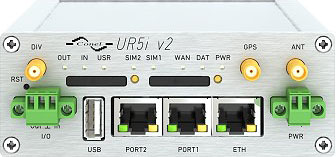
\includegraphics[width=.5\LW]{UR5i_v2}
    \caption{UR5i v2 v kovové krabici.}
    \label{fig:UR5i_v2}
  \end{subfigure}
  \begin{subfigure}[h]{0.5\LW}
    \centering
    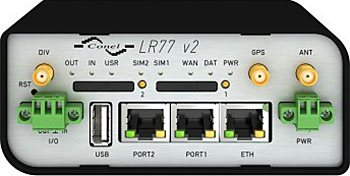
\includegraphics[width=.5\LW]{LR77_v2}
    \caption{LR77 v2 v plastové krabici.}
    \label{fig:LR77_v2}
  \end{subfigure}
  \caption{Příklad vzhledu řady routerů v2.}
  \label{fig:UR5i_v2}
\end{figure}

\subsection{Řada routerů v3}
Modelová řada v3 je poslední vyvinutou řadou routerů. Koncepčně se příliš nelíší od předchozí řady. Různé kombinace routerů lze tvořit pomocí dvou volitelných portů. Jednotlivé porty lze osadit jakýmkoliv volitelným portem, nebo deskou s bezdrátovým modulem. Aby bylo možné obsáhnout testování alespoň nabízených kombinací routerů, bude v testovací laboratoři muset běžet přibližně dvacet routerů této řady. V základní konfiguraci bude muset být navíc oproti v2 řadě testován jeden binární vstup a jedno ethernetové rozhraní.

\begin{figure}[h]
  \begin{subfigure}[h]{0.5\LW}
    \centering
    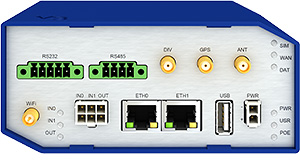
\includegraphics[width=.5\LW]{spectre_LTE}
    \caption{Spectre LTE v plastové krabici.}
    \label{fig:spectre_LTE}
  \end{subfigure}
  \begin{subfigure}[h]{0.5\LW}
    \centering
    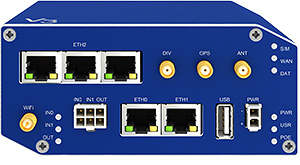
\includegraphics[width=.5\LW]{spectre_LTE_SL}
    \caption{Spectre LTE v kovové krabici.}
    \label{fig:spectre_LTE_SL}
  \end{subfigure}
  \caption{Příklad vzhledu řady routerů v3.}
  \label{fig:spectre_LTE}
\end{figure}

\section{Volitelné porty}
Každý router lze osadit alespoň jedním volitelným portem. Jednotlivé volitelné porty rozšiřují router o další interface. Testovány musí být všechny volitelné porty alespoň v každé modelové řadě routerů. Popis volitelných portů a způsob zapojení je popsán v kapitolech týkajících se jednotlivým volitelným portům.

\subsection{Ethernet 10/100}
Volitelný port Ethernet 10/100 rozšiřuje router o další fyzický ethernet rozhraní. Tento port bude testován stejný způsobem jako základní ethernet na routeru. Všechny tyto porty budou připojeny do konfigurovatelného switche a pomocí VLAN budou odděleny do jiné sítě.

\subsection{RS232}
Volitelný port RS232 rozšiřuje router o standartní sériové rozhraní. Sériová rozhraní budou testována trojím způsobem. Nejdříve budou propojeny dva routery sériovým rozraním a mezi nima budou přenášena data. Drůhým způsobem testů bude připojení loopback desky, která odpovídá na pár základních komandů. Například na příkaz ATI loopback deska odpovídá název testovaného rozhraní a hlášku OK. Poslední testovací případ sériového rozhraní bude připojení a komunikace s libovolným zařízením jiného výrobce.

\subsection{RS485/RS422}
Volitelný port RS485/RS422 rozšiřuje router o přepínatelné sériové rozhraní RS485 a RS422. Testování těchto portů je identické s rozhraním RS232. Testovat bude potřeba obě tyto rozhraní. Výběr jednoho z rozhraní je prováděno pomoci jumperů na desce volitelného portu.

\subsection{M-BUS master}
Volitelný port M-BUS master rozšiřuje router o další typ sériového rozhraní. Testování tohoto portu bude prováděno zapojením M-Bus slave loopback destičky. Druhým způsobem tesování bude zapojení reálného M-Bus měřáku. Reálné zařízení je vždy zapojeno pouze jedno v celém testlabu, do ostatních volitelných portů jsou zapojovány loopback desky.

\subsection{I/O module CNT}
Volitelný port I/O module CNT rozšiřuje router o další binární vstupy, binární výstupy, čítačové vstupy a analogové vstupy. Testování tohoto portu bude prováděno pouze jedním způsobem. Volitelný port CNT se bude testovat pomocí loopback desky CNT.

\subsection{WiFi}
Volitelný port WiFi rozšiřuje router o možnost připojení se do WiFi sítě. Tento rozšiřuící port lze osadit pouze do modelové řady v2. Řada routerů v1 nepodporuje WiFi rozhraní. Ŕada routerů v3 má možnost osadit WiFi rozhraní již na základní desce. WiFi rozhraní se bude testovat vůči WiFi připojení testovacího serveru, WiFi připojení CISCO routeru a v neposlední řadě vůči jinemů Conel routeru s podporou WiFi.

\subsection{SDH}
Volitelný port SDH rozšiřuje možnost routeru o připojení SD karty. Kompatibilita portu SDH je stejná jakou u portu WiFi. Testování portu SDH bude pomocí zápisu a přečtení dat z karty umístěné v držáku SDH portu. Źádná konektivita v případě tohoto portu nebude potřeba.

\subsection{Switch}
Volitelný port Switch rozšiřuje možnost připojení se až na tři switchované ethernet porty. Po připojení portu Switch do routeru je první ethernet switchován do všech tří portů routeru. Kompatibilita tohoto volitelného portu je stejná jako u předchozích dvou portů.

\section{Cisco router}
Další důležito součástí testovací sítě je bezdrátový Cisco router. Router je zapojen do testovací sítě pomocí ethernetu. Router dále využívá mobilní a WiFi připojení. Cisco router je součástí testovací sítě z důvodu testování vybraných protokolů oproti jinému referenčnímu routeru. Příklad testovaného protokolu může být například IPsec tunel.

\section{Další pomocné přístroje}
V testovací síti budou dále přibývat různá zařízení pro možnosti lepšího testování jednotlivých rozhraní všech router. Mezi tyto zařízení budou například patřit různé měřáky se sériovým rozhraním RS232, či M-BUS měřáky. Dále bude v testovací síti umístěny konkurenční výrobky pro ověření funkčnosti testovaných výrobků s jinými síťovými prvky.

\begin{figure}[h]
  \centering
  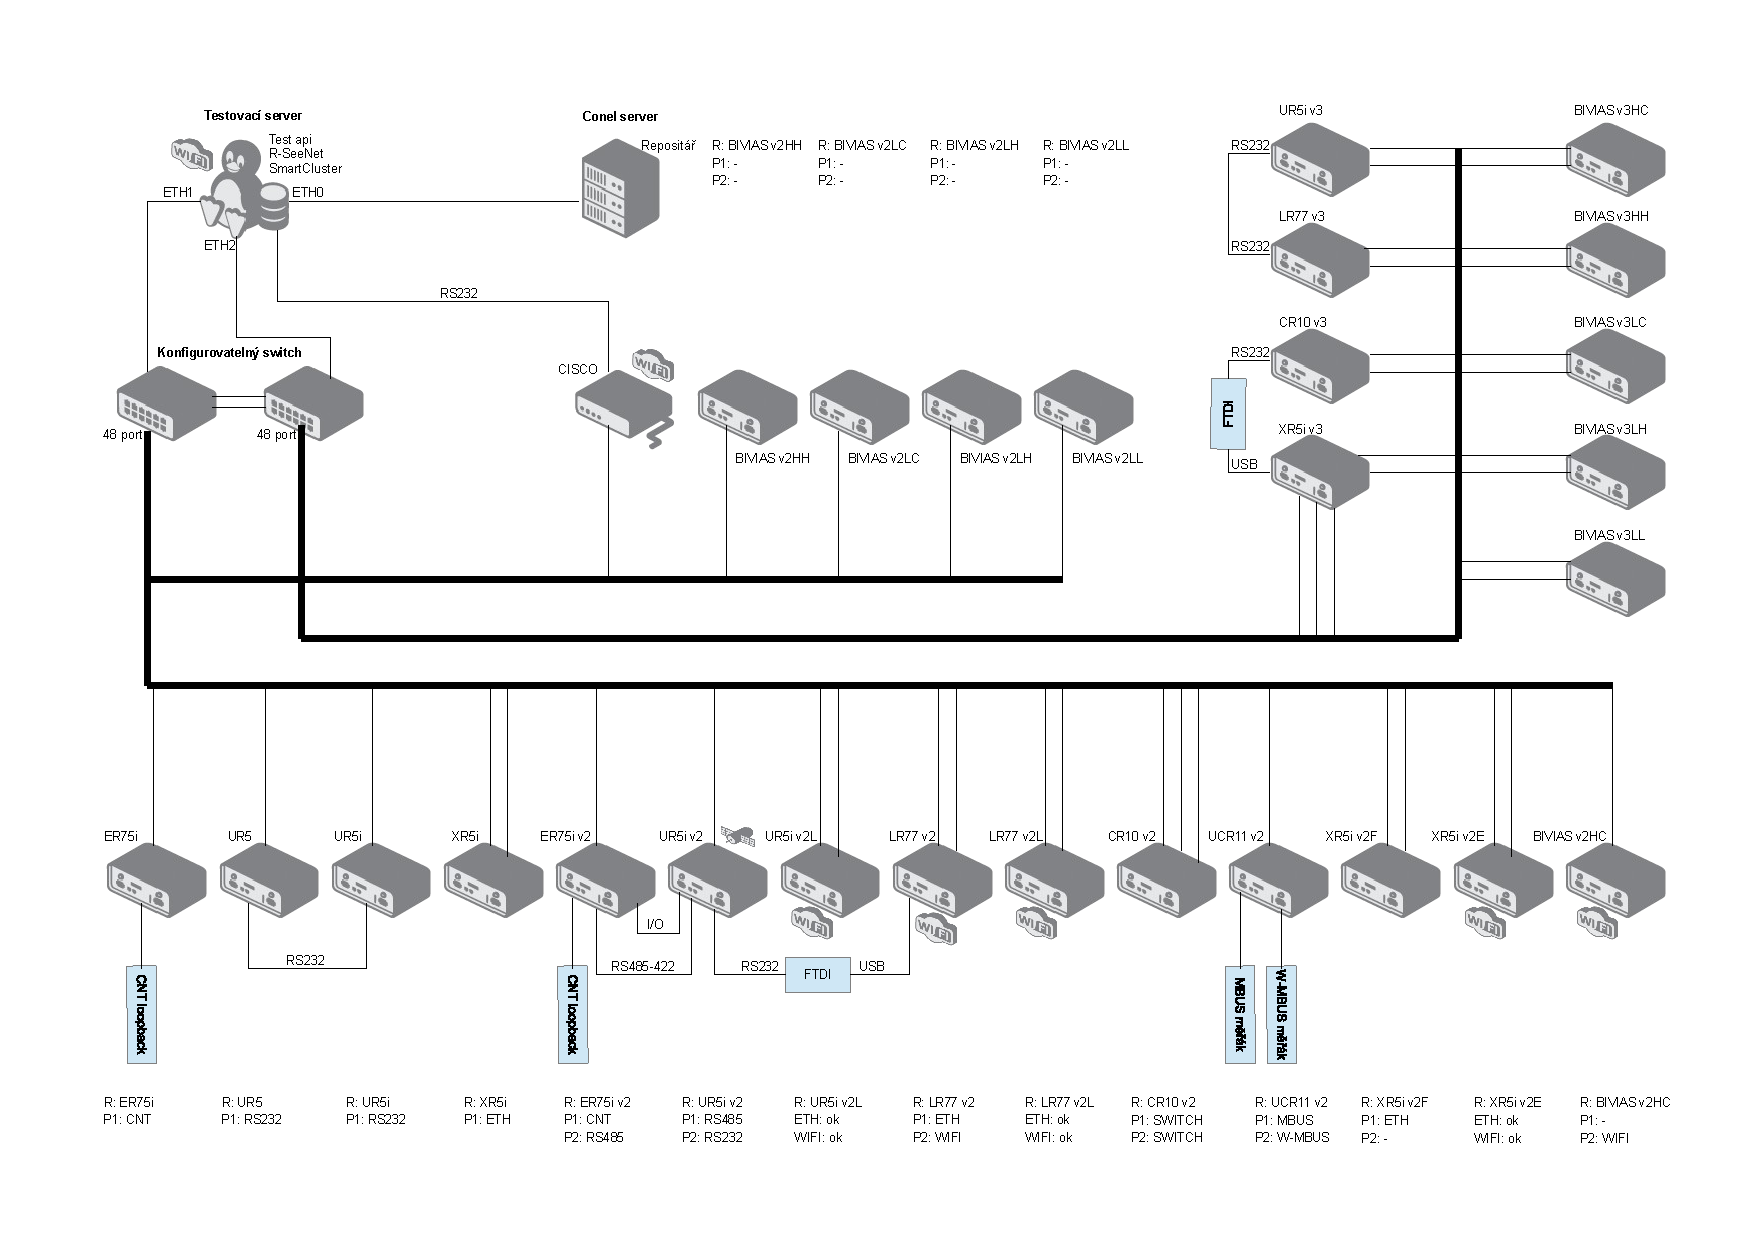
\includegraphics[angle=90,origin=c,width=\LW]{schema_site}
  \caption{Schéma testovací laboratoře}
  \label{fig:schema_site}
\end{figure}

\endinput
